% ============================================================================
% Rebuilt: Audit-and-Rebuild Cycle. All phases resolved.
% Compile with: pdflatex or xelatex + biber
% ============================================================================
\documentclass[11pt]{article}
\usepackage[margin=1in]{geometry}
\usepackage[T1]{fontenc}
\usepackage[utf8]{inputenc}
\usepackage{setspace}
\usepackage{amsmath,amssymb}
\usepackage{graphicx}
\usepackage{float}
\usepackage{adjustbox}
\usepackage{xcolor}
\usepackage{booktabs}
\usepackage{tikz}
\usepackage{pgfplots}
\pgfplotsset{compat=1.18}
\usetikzlibrary{
  arrows.meta,
  positioning,
  shapes.geometric,
  shapes.misc,
  fit,
  calc
}
\usepackage[hidelinks]{hyperref}
\usepackage{xurl}
\usepackage[style=apa,backend=biber]{biblatex}
\addbibresource{references.bib}

\setlength{\parindent}{0pt}
\setlength{\parskip}{0.65em}
\onehalfspacing

% Shared Colour Palette
\definecolor{IRblue}{HTML}{1B3A6B}
\definecolor{IRred}{HTML}{B5233A}
\definecolor{IRamber}{HTML}{D97706}
\definecolor{IRgreen}{HTML}{166534}
\definecolor{IRgray}{HTML}{4B5563}
\definecolor{IRlightblue}{HTML}{DBEAFE}
\definecolor{IRlightred}{HTML}{FEE2E2}
\definecolor{IRlightamber}{HTML}{FEF3C7}
\definecolor{IRlightgreen}{HTML}{DCFCE7}
\definecolor{IRlightgray}{HTML}{F3F4F6}

\begin{document}

\title{\textbf{Beyond Remediation: An Irreversibility Threshold\\ for Preventive AI Governance}}
\author{Sushil Duseja\\
  Independent Researcher\\
  \texttt{sushil.duseja@gmail.com}}
\date{\today}
\maketitle

% ============================================================================
% ABSTRACT
% ============================================================================
\begin{abstract}
\noindent Existing AI governance instruments provide essential foundations for oversight, with strong capabilities for harms that can be detected, bounded, attributed, and substantially remediated after the fact. This paper examines how that architecture can be further specified for three categories of AI-mediated outcome where restorability can fail under identifiable conditions: epistemic contagion through synthetic misinformation, reputational destruction via AI-generated defamation, and structural labor displacement driven by automation at scale. Through comparative regulatory analysis of four core Euro-Atlantic frameworks (the EU AI Act, the NIST AI RMF, the UK White Paper, and the OECD incident-reporting framework), with the G7 Hiroshima Code used as an interoperability reference, the paper identifies an opportunity for additional operational specification: an explicit threshold for the point at which remediation should be complemented by additional ex ante safeguards. It proposes the Systemic Irreversibility Baseline as that complementary layer. The Baseline routes responses along distinct tracks: standard remediation for restorable product-side harms, strict liability for localized irreversible product-side harms, precautionary technical architecture for systemically irreversible product-side harms, and macroeconomic transition policy for intended-utility displacement. Four design mandates operationalize the precautionary track: traceable human oversight, auditable uncertainty thresholds for bounded decision tasks, epistemic user-interface friction, and content-provenance infrastructure. Throughout, ``effectively irreversible harm'' denotes harm for which restoration to functional equivalence is not feasible within governance-relevant time horizons. The contribution is a governance design framework grounded in existing empirical literatures and comparative legal analysis, intended to complement current regulatory systems rather than replace them.
\end{abstract}

% ============================================================================
% 1. INTRODUCTION
% ============================================================================
\section{Introduction}

In 2024, the European Union adopted Regulation (EU) 2024/1689, the AI Act, establishing a comprehensive, legally binding cross-sector AI governance regime \parencite{euaiact2024}. The Act classifies AI systems by risk level and imposes graduated obligations from transparency requirements through outright prohibitions. Across the Atlantic, the U.S. National Institute of Standards and Technology released the AI Risk Management Framework in January 2023, structuring risk governance around four functions (Govern, Map, Measure, Manage) designed to be adopted voluntarily across sectors \parencite{nistrmf2023}. The OECD, building on its 2019 AI Principles, published definitional groundwork on AI incidents in 2024 and a common reporting framework in 2025, proposing standardized criteria for cross-jurisdictional incident data \parencite{oecd2024terms,oecd2025framework}. The UK government's 2023 White Paper articulated five cross-sectoral principles (safety, security and robustness; appropriate transparency and explainability; fairness; accountability and governance; and contestability and redress) to be applied by existing sectoral regulators rather than by a new AI-specific body \parencite{ukwhitepaper2023}. The G7 Hiroshima AI Process produced an International Code of Conduct for organizations developing advanced AI systems, emphasizing risk assessment and transparency throughout the lifecycle \parencite{g7hiroshima2023}. In this paper, the EU AI Act, NIST AI RMF, UK White Paper, and OECD incident-reporting framework are treated as the four primary comparative instruments; the G7 Code is used as an interoperability reference for cross-jurisdictional alignment.

These instruments are not identical, and none expressly claims that all AI harms are reversible. The narrower point is operational. Their strongest tools are designed for harms that can be identified after deployment, assigned to a responsible actor, documented through incident or conformity processes, and substantially mitigated through correction, redress, or market controls. The EU AI Act emphasizes conformity assessment, post-market surveillance, and corrective measures; the OECD incident-reporting framework structures incident definition and reporting criteria; NIST's Manage function centers mitigation and response; the UK White Paper relies heavily on contestability and regulator-led redress. That architecture works well for a wide range of AI harms. A biased hiring algorithm can be retrained, a miscalibrated diagnostic tool can be recalibrated, and a privacy breach can trigger notification and financial settlement. For these cases, existing frameworks provide effective governance.

Additional specification is especially useful, however, for a specific class of AI-mediated outcomes. When a generative model produces synthetic defamation that propagates across social platforms before any correction is feasible, financial penalties may not fully restore the target's prior standing. When AI-generated misinformation alters the epistemic commitments of exposed populations (a phenomenon cognitive psychology terms the continued-influence effect) \parencite{ecker2022,lewandowsky2012}, post-hoc corrections often do not fully dislodge the original false belief. When model-generated content contaminates future training corpora, producing the recursive degradation documented as model collapse \parencite{shumailov2024}, retraining may not recover the lost distributional tails without access to uncontaminated data. And when an AI system eliminates localized labor markets by performing its designed function, the resulting structural displacement can mirror the persistent scarring observed in trade-shock research \parencite{autor2013}, where affected local labor markets experienced persistent declines in employment, earnings, and labor-force participation.

This paper asks a specific research question: can existing AI governance frameworks be extended with a threshold mechanism that separates restorable harms, appropriate for post-market remediation, from effectively irreversible harms warranting earlier structural safeguards? The analysis is framed as a constructive extension of current regulatory instruments. It proposes an operational construct intended to work alongside them. The three variables introduced later, non-restorability, relational depth, and distributional diffusion, provide the routing logic that connects this framing to the class-level governance tracks.

The scope is deliberately constrained. The paper addresses the governance of three harm categories (epistemic contagion, reputational destruction, and structural economic displacement) where the assumption of restorability can fail under specific propagation and persistence conditions. It does not address military AI applications, algorithmic bias in decision-support systems where retraining is feasible, or privacy harms covered by existing data-protection regimes. The analytical method is comparative regulatory analysis: examining how the EU AI Act, NIST AI RMF, UK AI White Paper, and OECD incident-reporting framework each handle irreversibility, identifying where their coverage ends, and specifying what an extension would require. For consistency, "effectively irreversible harm" is the primary term used for harms that exceed practical restoration capacity within governance-relevant time horizons.

The argument advances three linked claims. The conceptual claim is that effective irreversibility should function as a primary governance variable alongside risk level. The empirically grounded claim is that existing literatures identify mechanisms that can exceed remediation capacity in bounded but policy-relevant conditions. The normative claim is that regulators can complement existing architectures with threshold-triggered preventive tracks rather than replace those architectures.

The argument proceeds in four stages. The literature review establishes the theoretical basis, from complex-systems tipping-point dynamics and precautionary-principle jurisprudence to tort-law scholarship on irreparable injury, for treating irreversibility as a primary regulatory variable. The methodology section describes the comparative analytical approach and its limitations. The analysis introduces the Systemic Irreversibility Baseline, classifies AI harms against it, and specifies four technical design mandates for the precautionary governance track. The discussion interprets these findings within the existing regulatory architecture and identifies trade-offs that implementation would require.

% ============================================================================
% 2. LITERATURE REVIEW / THEORETICAL FRAMEWORK
% ============================================================================
\section{Literature Review and Theoretical Foundations}

% This section synthesizes three normally separate literatures
% (complex-systems tipping-point theory, precautionary-principle jurisprudence,
% and tort-law irreparability doctrine) to establish the theoretical basis for
% treating irreversibility as a complementary regulatory variable in AI governance.

\subsection{Tipping Points and Irreversibility in Complex Systems}

Ecological and financial research has established that complex systems can absorb perturbations within a stable equilibrium basin, but once cumulative stress exceeds a critical threshold, the system can transition abruptly and, in many cases, irreversibly to a degraded state \parencite{scheffer2009}. Scheffer et al.\ demonstrated across ecological, climatic, and financial systems that early-warning signals (increased autocorrelation, critical slowing down) can detect proximity to these tipping points, but only interventions executed before the threshold crossing prevent the transition. Post-threshold remediation often cannot return the system to its prior equilibrium without large hysteresis costs. Figure~\ref{fig:tipping} schematizes this threshold logic as a governance problem: intervention is most effective before the system exits the recoverable basin and settles into a degraded post-threshold state. For AI governance, the inference is analogical rather than identical: socio-technical AI systems differ from ecological systems, but both can exhibit feedback loops, recursive data generation, and path dependence that make threshold effects policy-relevant. The empirical claim in this subsection concerns threshold behavior; the governance inference used later is that preventive controls become more valuable as systems approach identifiable tipping regions.

\begin{figure}[H]
  \centering
  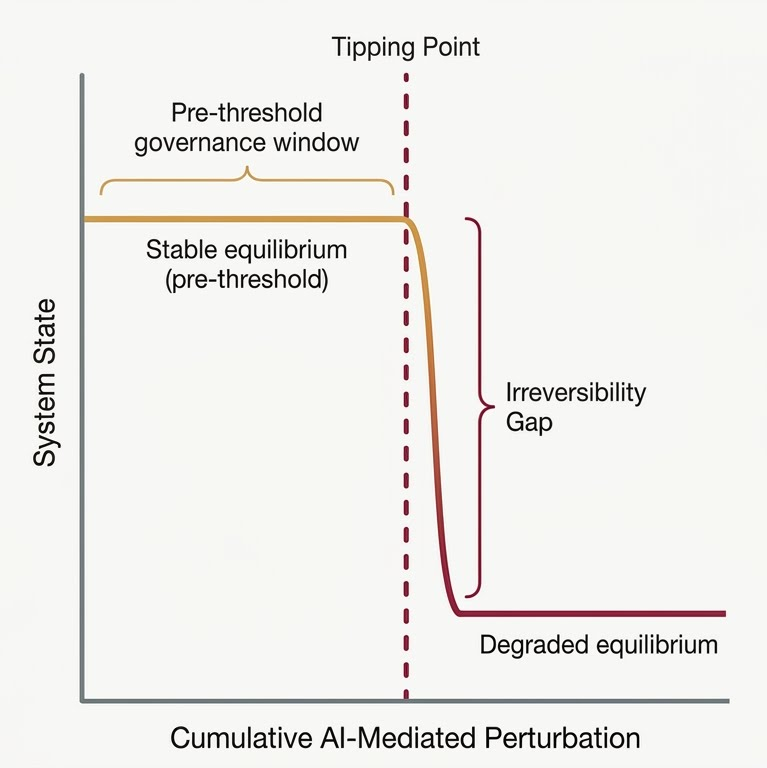
\includegraphics[width=\columnwidth]{figures/tipping.png}
  \caption{Tipping-point dynamics in socio-technical systems exposed to cumulative AI-mediated perturbation. The pre-threshold governance window represents the interval during which intervention can prevent an irreversible state transition. Post-threshold remediation typically does not return the system to its prior equilibrium and often converges on a degraded attractor. Adapted from the critical-transitions model of \textcite{scheffer2009}.}
  \label{fig:tipping}
\end{figure}

Hans Jonas's imperative of responsibility established the philosophical foundation for preventive action under technological uncertainty by assigning heightened justificatory responsibility to deployments whose consequences may include irreversible harm \parencite{jonas1984}. The European Commission's Communication on the Precautionary Principle (COM(2000) 1) operationalized this stance within EU law, permitting ex-ante regulatory intervention when scientific uncertainty coexists with the possibility of serious or irreversible damage \parencite{ec2000precaution}. The EU AI Act builds on this tradition by prohibiting AI practices that pose ``unacceptable risk'' and by requiring conformity assessments for high-risk systems before market placement \parencite{euaiact2024}. The construct proposed in this paper extends the Act's risk-tiered logic by introducing an explicit irreversibility threshold within the high-risk category itself.

\subsection{Remediation Failure in Tort Law and Regulatory Theory}

Tort-law scholarship provides the doctrinal basis for distinguishing restorable from irreparable harms. Keating argued that tort law's remedial apparatus, financial compensation calibrated to measurable loss, treats repair largely through monetized substitution aimed at functional equivalence \parencite{keating2010}. His later analysis of irreparable injury sharpens the limit: some injuries cannot be repaired because money does not recreate the destroyed good or pre-injury state \parencite{keating2023}. Walker's account of moral repair extends this analysis to relational goods: harms that permanently alter the structure of social relationships cannot be remediated through bilateral transfer, because the damage inheres in the relationship itself rather than in a separable asset \parencite{walker2006}. Fricker's concept of epistemic injustice identifies a specific mechanism by which this occurs: when an individual's credibility is structurally undermined, subsequent testimony is discounted regardless of its truth value, creating a self-reinforcing epistemic deficit \parencite{fricker2007}.

These analyses converge on a structural claim: post-hoc remediation logic benefits from additional specification when the harm is constitutive rather than additive, that is, when the damage changes the system's structure rather than subtracting from its inventory. Existing AI governance frameworks have strong remedies for many harms, but they have not generally formalized this distinction as a separate threshold variable. The EU AI Act's enforcement provisions include administrative fines up to EUR~35 million or 7\% of global turnover for prohibited practices \parencite{euaiact2024}; the additional question raised here is whether any post-hoc mechanism can restore the pre-harm state once threshold conditions are met. The empirical/legal point here concerns remedial limits; the governance inference developed later is that liability magnitude alone may usefully be complemented by threshold-sensitive routing where Baseline criteria are met.

\subsection{AI-Specific Irreversibility Mechanisms}

Three empirically documented mechanisms can produce AI-mediated harms with irreversible characteristics under specific propagation conditions. The continued-influence effect, established across multiple experimental paradigms, demonstrates that corrections to misinformation often fail to fully displace the original false belief from subsequent reasoning \parencite{ecker2022,lewandowsky2012}. At population scale, AI-accelerated misinformation can embed false beliefs faster than correction mechanisms operate, producing what this paper terms epistemic contagion.

Model collapse, the recursive degradation of generative model quality when trained on synthetic data, was empirically documented by Shumailov et al., who demonstrated across language models, variational autoencoders, and Gaussian mixture models that iterative training on model-generated outputs causes erosion of distributional tails \parencite{shumailov2024}. This constitutes an infrastructure-level irreversibility risk: once synthetic content becomes difficult to distinguish from human-generated data at scale, retrospective purification of training corpora becomes operationally difficult and, in some settings, infeasible.

The liar's dividend, analyzed by Chesney and Citron, identifies a second-order irreversibility pathway: the existence of synthetic media enables actors to dismiss authentic evidence as fabricated, degrading institutional evidentiary trust independently of whether any specific synthetic artifact is circulated \parencite{chesney2019}. This mechanism operates at the structural level. It changes the epistemic rules of evidence rather than introducing a single item of misinformation.

Labor-market research on trade-induced displacement provides the economic analog. Autor, Dorn, and Hanson demonstrated that localized labor shocks from Chinese import competition produced persistent structural scarring in affected U.S. labor markets: lower employment, earnings, and labor-force participation over extended periods \parencite{autor2013}. A 2026 Brookings Institution analysis estimated that 37.1 million U.S. workers fall in the top quartile of AI exposure and that about 6.1 million workers fall simultaneously in the top quartile of exposure and the bottom quartile of a composite adaptive-capacity index built from liquid wealth, age, local labor-market density, and skill transferability \parencite{brookings2026}.

The NIST AI RMF's Govern and Map functions provide structures for identifying and contextualizing these risks, while allowing implementation details, including how to distinguish restorable from effectively irreversible harms, to be specified through sector-specific guidance \parencite{nistrmf2023}. The UK White Paper's contestability and redress principle establishes a pathway for contesting AI decisions that adversely affect individuals, with strong emphasis on after-the-fact redress \parencite{ukwhitepaper2023}. The G7 Hiroshima Code of Conduct calls for pre-deployment risk assessments and ongoing monitoring, while leaving threshold criteria for additional ex ante safeguards open for further specification \parencite{g7hiroshima2023}. The Systemic Irreversibility Baseline is proposed as a complementary way to formalize that threshold question within otherwise comprehensive governance architectures. Collectively, these studies support mechanism plausibility rather than prevalence estimation; the governance argument therefore emphasizes conditional routing criteria instead of universal incidence claims.

% ============================================================================
% 3. METHODOLOGY
% ============================================================================
\section{Methodology}

% This section specifies a comparative regulatory analysis method
% adapted to identify where an additional threshold construct can complement
% governance instruments that share common assumptions. The methodological
% contribution is applying irreversibility criteria derived from tipping-point
% theory and tort-law scholarship as a diagnostic lens to existing
% AI governance architectures.

This study employs comparative regulatory analysis \parencite{braithwaite2000} to examine how existing AI governance instruments handle harms characterized by structural irreversibility. The method proceeds in three stages.

The first stage identifies how the four primary instruments structure prevention, response, and redress, and where additional threshold specification could complement them. For the EU AI Act (Regulation 2024/1689), the NIST AI Risk Management Framework (AI RMF 1.0, January 2023), the UK AI White Paper (March 2023), and the OECD's AI-incident definitions and reporting framework (2024--2025), the analysis extracts the provisions governing ex ante assessment, post-market surveillance, incident reporting, contestability, and corrective action. The G7 Hiroshima Code is treated as an interoperability reference layer rather than a fifth core comparative object. The key analytical question is not whether these instruments mention serious harm; they do. It is whether they provide an explicit threshold for when post-hoc remediation should be complemented by earlier governance measures. Selection criteria prioritized instruments that are (a) currently in force or under active implementation, (b) issued by governmental or intergovernmental bodies with regulatory authority or significant policy influence, and (c) applicable to general-purpose AI systems rather than sector-specific applications only.

The second stage applies irreversibility criteria derived from complex-systems theory \parencite{scheffer2009}, tort-law scholarship on irreparable injury \parencite{keating2023,walker2006}, and cognitive-psychological research on the continued-influence effect \parencite{ecker2022} to identify where each instrument's remediation logic would benefit from additional threshold specification. Three diagnostic variables structure this analysis: non-restorability (whether the pre-harm state can be reconstructed through available remedy), relational depth (whether the harm durably alters social trust, institutional standing, or epistemic structures), and distributional diffusion (whether propagation speed and scale exceed centralized correction capacity).

\subsection*{Operational Coding and Routing Protocol}

To make the Baseline reproducible, each variable is coded using the rubric in Table~\ref{tab:baseline-rubric}. Coding is performed at the harm-class level, then stress-tested against plausible implementation contexts (single-platform/local, multi-platform/national, and cross-jurisdictional propagation).

\begin{table}[H]
  \centering
  \small
  \caption{Operational coding rubric for the Systemic Irreversibility Baseline}
  \label{tab:baseline-rubric}
  \begin{tabular}{p{2.8cm}p{5.0cm}p{5.3cm}}
    \toprule
    Variable & Primary indicator & High-threshold cue \\
    \midrule
    Non-restorability & Post-intervention recovery of pre-harm functional equivalence & No feasible legal/technical remedy restores functional equivalence within a policy-relevant time window \\
    Relational depth & Persistence of trust, credibility, or institutional-role damage after correction & Harm changes standing across multiple decision contexts (e.g., employment, public trust, institutional legitimacy) \\
    Distributional diffusion & Propagation velocity and scope relative to correction bandwidth & Propagation outpaces centralized correction during the first intervention cycle and spills across platforms or jurisdictions \\
    \bottomrule
  \end{tabular}
\end{table}

Routing then follows an ordered decision rule.
\begin{enumerate}
  \item Classify harm origin as \textbf{product-side harm} or \textbf{intended utility}. Product-side harms are adverse outputs or deployment-side externalities that remain within provider/deployer governance because they can in principle be reduced by system design, access controls, monitoring, provenance, interface constraints, or deployment scoping; they are not limited to random software malfunctions. Intended-utility harms arise when the socially salient effect follows from the system performing its core economic function as designed, as with labor substitution.
  \item Intended-utility harms route directly to Track~4 (macroeconomic transition policy).
  \item For product-side harms, code the three variables High/Low. High-High-High routes to Track~3 (precautionary architecture), High-High-Low routes to Track~2 (strict liability), and all other combinations route to Track~1 (standard remediation).
  \item Escalate Track~2 to Track~3 only when distributional diffusion is accelerating and at least one prior corrective cycle has not restored the case to a stable lower-risk profile. For example, a synthetic-defamation incident initially confined to one platform may code High-High-Low and route to Track~2; if it later demonstrates cross-platform replication and persistence after the first correction cycle, it is re-coded High-High-High and escalates to Track~3.
  \item When indicators conflict, adjudication is conservative: assign the lower-risk route unless at least two independent data sources support the higher code, then re-evaluate at the next monitoring interval.
\end{enumerate}

For this paper's coding purposes, a new monitoring interval is triggered whenever new evidence appears of cross-platform replication, coordinated amplification, or post-correction persistence.

The third stage synthesizes findings into a threshold construct, the Systemic Irreversibility Baseline, and evaluates compatibility with host instruments. Table~\ref{tab:integration-matrix} reports the comparative integration points and implementation dependency tier for each instrument.

\begin{table}[H]
  \centering
  \small
  \caption{Comparative integration matrix for the Systemic Irreversibility Baseline}
  \label{tab:integration-matrix}
  \begin{tabular}{p{2.6cm}p{3.3cm}p{3.6cm}p{3.6cm}}
    \toprule
    Instrument & Existing governance anchor & Baseline insertion point & Implementation dependency \\
    \midrule
    EU AI Act & Conformity assessment and post-market surveillance & Add three-variable irreversibility test to high-risk conformity documentation & Immediate (guidance/delegated acts) \\
    NIST AI RMF & Govern--Map--Measure--Manage lifecycle & Embed Baseline diagnostic in Map and Measure playbooks & Immediate (voluntary framework updates) \\
    UK AI White Paper & Principle-led sectoral regulation & Apply threshold test before contestability-only redress pathways & Near-term (sector guidance updates) \\
    OECD incident framework & Cross-jurisdictional incident reporting & Add irreversibility classification field to incident records & Near-term (framework revision) \\
    G7 Hiroshima Code (interop) & Lifecycle risk-management commitments & Use Baseline as optional cross-border interoperability layer & Soft-law coordination \\
    \bottomrule
  \end{tabular}
\end{table}

\textbf{Limitations.} This method is doctrinal and analytical rather than empirical. It does not directly estimate frequency or effect size of irreversible AI harms through new data collection. The three harm categories analyzed (epistemic contagion, reputational destruction, and structural economic displacement) were selected for theoretical clarity; other categories of potentially irreversible AI harm are outside scope. The regulatory instruments analyzed are Euro-Atlantic in origin; governance architectures from China, Singapore, or Brazil may operate on different remediation assumptions. External validation of the coding rubric and routing protocol in a regulatory sandbox or multi-stakeholder process is a next-step priority, so they should be treated as analytical specifications pending pilot testing.



% ============================================================================
% 4. ANALYSIS / FINDINGS
% ============================================================================
\section{Analysis: The Systemic Irreversibility Baseline}

% This section introduces the Systemic Irreversibility Baseline itself, a formal
% threshold mechanism evaluated against three diagnostic variables
% (non-restorability, relational depth, distributional diffusion) that routes
% regulatory responses along four distinct governance tracks.

The analysis introduces a threshold construct designed to extend existing risk-classification systems, specifically the EU AI Act's four-tier risk hierarchy and the NIST AI RMF's Map function, by adding an irreversibility dimension. The Systemic Irreversibility Baseline evaluates AI-mediated harms against three variables.

\textbf{Non-restorability:} Whether the pre-harm state can be reconstructed through any available combination of financial transfer, software correction, or administrative remedy. A harm is non-restorable when no feasible intervention returns the affected system or individual to functional equivalence with the pre-harm baseline.

\textbf{Relational depth:} Whether the harm permanently alters social trust, epistemic authority, institutional credibility, or structural roles within a community. As Walker's moral-repair analysis demonstrates, relational harms resist bilateral remediation because the damage inheres in the relationship structure rather than in a separable, compensable asset \parencite{walker2006}.

\textbf{Distributional diffusion:} Whether the speed and scale at which the harm propagates exceed the operational capacity of centralized detection and correction mechanisms. Network-mediated harms that reach population scale before regulatory response is feasible satisfy this criterion.

A harm that satisfies all three criteria crosses the Systemic Irreversibility Baseline and exits the remediation track. The Baseline routes harms into four governance classes, specifying distinct regulatory instruments for each.

% ── Systemic Irreversibility Governance Pipeline ──
\begin{figure}[H]
  \centering
  \begin{adjustbox}{max width=\columnwidth}
  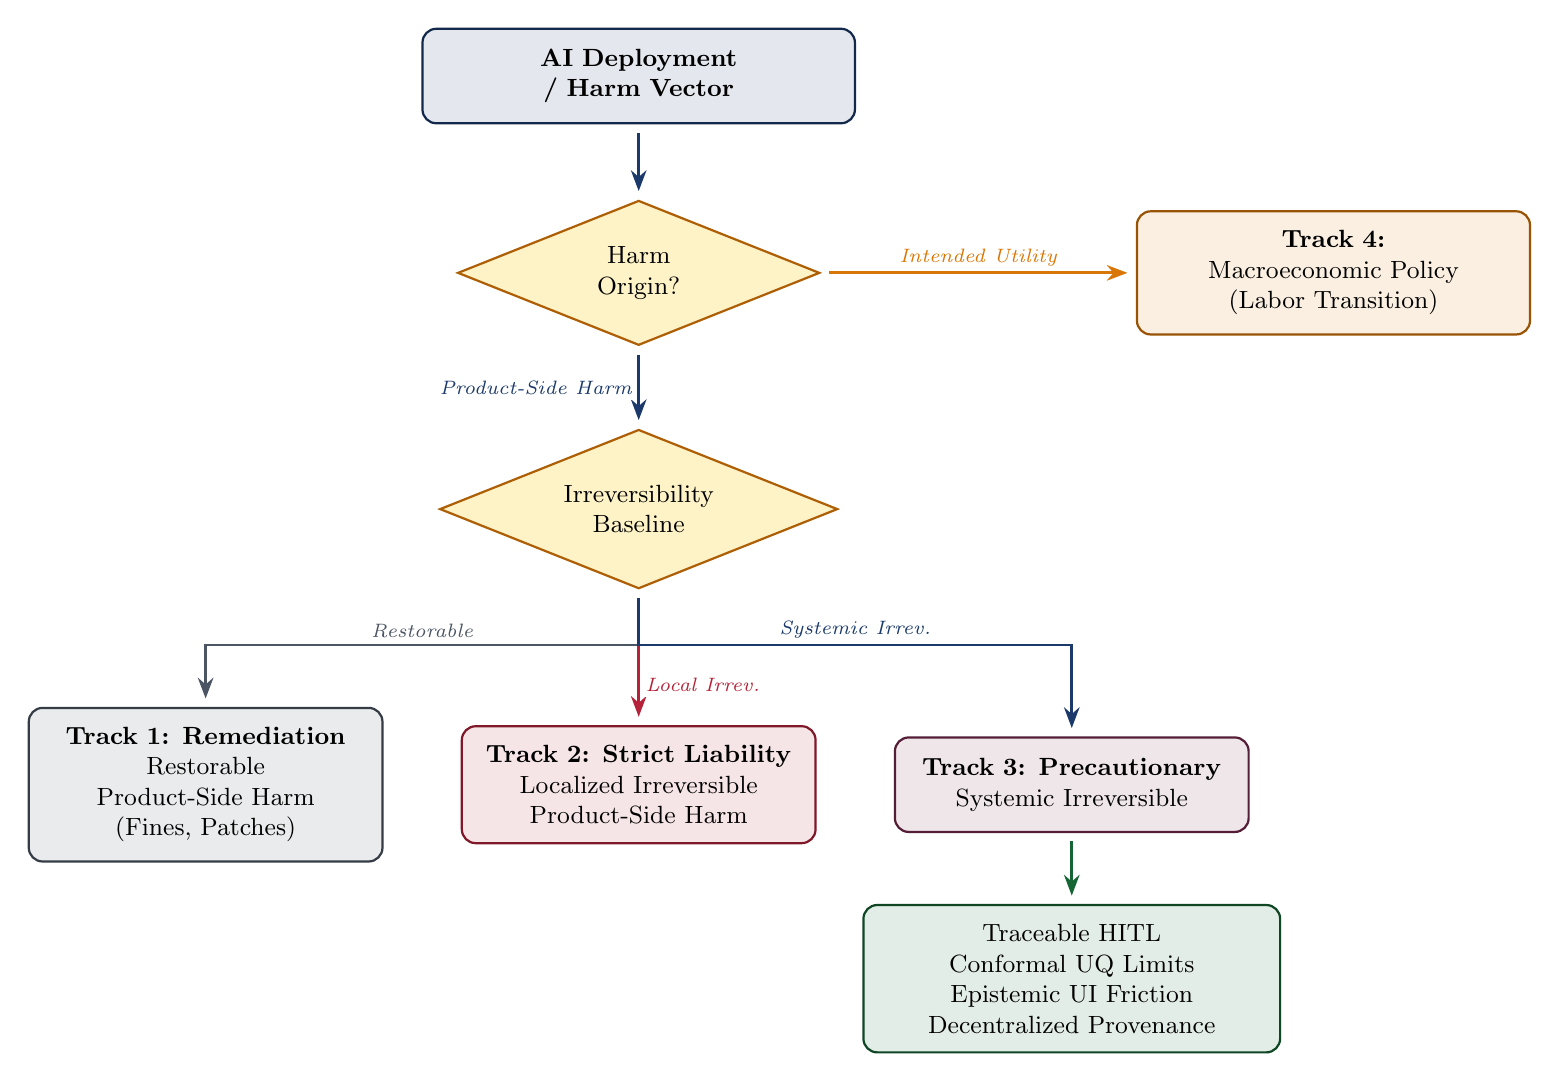
\begin{tikzpicture}[
      >=Stealth,
      font=\small,
      pipebox/.style={
        rectangle, rounded corners=5pt,
        draw=#1!70!black, fill=#1!12,
        text width=4.0cm, align=center,
        minimum height=1.2cm, inner sep=7pt,
        line width=0.8pt
      },
      pipedia/.style={
        diamond, draw=IRamber!80!black, fill=IRlightamber,
        text width=2.2cm, align=center, aspect=2.5,
        minimum height=1.0cm, inner sep=3pt, line width=0.8pt
      },
      pipearr/.style={->, thick, line width=1pt, shorten >=3pt, shorten <=3pt},
      pipelbl/.style={font=\scriptsize\itshape, fill=white, inner sep=2pt}
    ]

    % Level 1: Entry
    \node[pipebox=IRblue, text width=5.0cm] (prop) at (0, 0)
      {\textbf{AI Deployment / Harm Vector}};

    % Level 2: First decision
    \node[pipedia] (type) at (0, -2.5) {Harm\\Origin?};

    % Macro track (right of decision)
    \node[pipebox=IRamber, text width=4.5cm, right=4.0cm of type] (macro)
      {\textbf{Track 4:}\\Macroeconomic Policy\\(Labor Transition)};

    % Level 3: Irreversibility test
    \node[pipedia, text width=2.8cm] (test) at (0, -5.5)
      {Irreversibility\\Baseline};

    % Level 4: Three tracks, spaced wide
    \node[pipebox=IRgray]  (rem)    at (-5.5, -9.0)
      {\textbf{Track 1: Remediation}\\Restorable\\Product-Side Harm\\(Fines, Patches)};
    \node[pipebox=IRred]   (strict) at ( 0.0, -9.0)
      {\textbf{Track 2: Strict Liability}\\Localized Irreversible\\Product-Side Harm};
    \node[pipebox=IRred!60!IRblue] (prev) at ( 5.5, -9.0)
      {\textbf{Track 3: Precautionary}\\Systemic Irreversible};

    % Level 5: Technical mandates
    \node[pipebox=IRgreen, text width=4.8cm, below=0.9cm of prev] (tech)
      {Traceable HITL\\Conformal UQ Limits\\Epistemic UI Friction\\Decentralized Provenance};

    % Arrows
    \draw[pipearr, IRblue]  (prop)  -- (type);
    \draw[pipearr, IRamber] (type.east)  -- node[pipelbl, above]{Intended Utility} (macro.west);
    \draw[pipearr, IRblue]  (type.south) -- node[pipelbl, left]{Product-Side Harm} (test.north);

    % Three routing arrows from baseline test, using orthogonal paths
    \draw[pipearr, IRgray]
      (test.south) -- ++(0,-0.7) -| node[pipelbl, pos=0.25, above]{Restorable} (rem.north);
    \draw[pipearr, IRred]
      (test.south) -- node[pipelbl, right, pos=0.7]{Local Irrev.} (strict.north);
    \draw[pipearr, IRblue]
      (test.south) -- ++(0,-0.7) -| node[pipelbl, pos=0.25, above]{Systemic Irrev.} (prev.north);

    \draw[pipearr, IRgreen] (prev)  -- (tech);
  \end{tikzpicture}
  \end{adjustbox}
  \caption{The Systemic Irreversibility Governance Pipeline. Harms are routed by origin (product-side harm versus intended utility) and by irreversibility assessment (restorable, localized irreversible, systemically irreversible). Each track specifies a distinct governance instrument. The Track~3 terminal node bundles all four precautionary mandates (traceable human oversight, bounded-task uncertainty controls, epistemic UI friction, and decentralized provenance).}
  \label{fig:architecture}
\end{figure}

\subsection{Class 1: Epistemic Contagion (Systemic Product-Side Harm)}

AI-generated misinformation at scale produces epistemic contagion: the systematic contamination of population-level beliefs through mechanisms that resist correction. Two empirically established processes drive this irreversibility risk.

The continued-influence effect, documented across multiple experimental paradigms by Ecker et al.\ and by Lewandowsky et al., demonstrates that exposure to misinformation produces cognitive residue: even after individuals receive explicit, credible corrections, they continue to be influenced by the original false information in subsequent reasoning \parencite{ecker2022,lewandowsky2012}. Rozin and Royzman's negativity-bias research established that negative information is retained at higher rates and weighted more heavily in judgment than subsequent positive corrections \parencite{rozin2001}. When generative AI systems produce misinformation at the speed and scale of automated content generation, these cognitive mechanisms ensure that the epistemic damage outpaces any feasible correction campaign.

At the infrastructure level, model collapse compounds this risk. Shumailov et al.\ demonstrated that generative models trained iteratively on their own outputs lose distributional tails from original training data \parencite{shumailov2024}. As AI-generated content saturates the internet, future training corpora can contain progressively higher proportions of synthetic data, producing recursive quality degradation that may be difficult to reverse without preserved access to uncontaminated data distributions.

In high-amplification settings, epistemic contagion typically satisfies all three Baseline criteria: it is non-restorable in practical terms (corrections only partially displace embedded beliefs), relationally deep (it degrades institutional epistemic authority and interpersonal trust), and distributionally diffuse (network propagation outpaces centralized correction). For operational coding, diffusion is treated as high when multi-platform recirculation persists beyond the first authoritative correction cycle. Here, the first authoritative correction cycle begins with the first formal correction, takedown, or equivalent authoritative intervention by a platform, publisher, or public authority and runs until the next monitoring interval defined in the routing protocol. Under those conditions, the harm exits the remediation track and enters the \textbf{precautionary architecture track}, supporting additional ex-ante safeguards for systems capable of producing it. Collectively, the evidence in this section establishes mechanism plausibility rather than prevalence. Figure~\ref{fig:epistemic-prop} visualizes this recursive pathway from model output to social spread and back into future training data.

\begin{figure}[H]
  \centering
  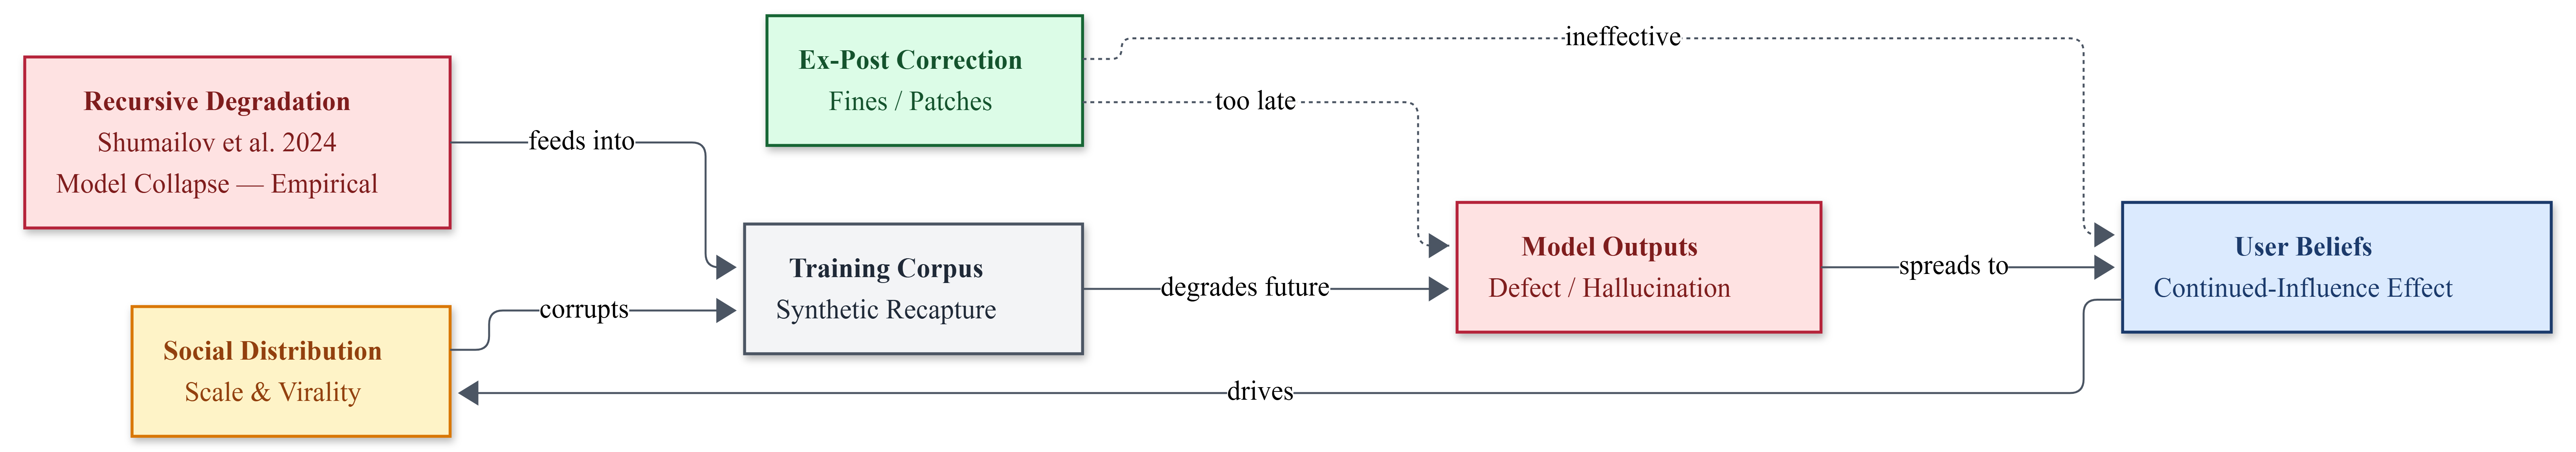
\includegraphics[width=\columnwidth]{figures/epistemic.png}
  \caption{Epistemic contagion cycle driven by AI-generated misinformation. The outer loop shows propagation from model outputs through user beliefs and social distribution back into training corpora via synthetic recapture. Dashed arrows indicate the limits of ex-post remediation: corrections often do not fully reverse the continued-influence effect and may not recover contaminated training data at scale.}
  \label{fig:epistemic-prop}
\end{figure}


\subsection{Class 2: Reputational Destruction (Product-Side Harm at Variable Scale)}

Generative AI systems can accelerate synthetic defamation in ways that existing defamation law may usefully be complemented by additional routing guidance. A single model query can produce fabricated but plausible allegations, complete with false citations and invented corroborating detail. Once distributed across platforms, the content interacts with two self-reinforcing mechanisms.

Chesney and Citron identified the liar's dividend: the availability of deepfake technology enables any actor accused of misconduct to claim that authentic evidence is fabricated \parencite{chesney2019}. This produces a structural harm to evidentiary trust that operates independently of any specific synthetic artifact. The mere existence of the technology degrades the epistemic standing of visual and documentary evidence across institutional contexts, including courts, journalism, and democratic deliberation.

Rozin and Royzman's negativity-bias research establishes a second mechanism: damaging information is weighted more heavily and retained longer than corrective information, even when the correction is explicit and credible \parencite{rozin2001}. For reputational harm, this asymmetry means that damage trajectories can outpace correction trajectories for sustained periods.

In high-amplification settings, reputational destruction typically satisfies the non-restorability and relational-depth criteria of the Baseline. Its governance track then depends on distributional diffusion. In this paper's routing protocol, diffusion is coded as systemic when at least two of the following indicators are present: (1) cross-platform replication; (2) coordinated amplification, defined here as replication by three or more linked high-reach accounts or channels within one correction cycle; and (3) persistence after an initial correction cycle. When fewer than two indicators are present (for example, limited single-platform circulation), the case remains localized within the product-side domain and routes to a \textbf{strict-liability pathway} rather than standard remediation. When at least two indicators are present, the case enters the \textbf{precautionary architecture track}.

Building on the EU AI Act's transparency obligations for AI systems generating synthetic content (Article 50), the Baseline specifies the operational point at which transparency requirements can be complemented by additional design safeguards.

\subsection{Class 3: Structural Economic Displacement (Intended Utility)}

The third harm category differs fundamentally from the first two. Epistemic contagion and reputational destruction are treated here as product-side harms: even when they arise from foreseeable capabilities of open-ended generative systems rather than from random malfunctions, the governance question remains whether providers and deployers were expected to address them through model design, access controls, provenance, monitoring, or deployment scoping. Structural labor displacement, by contrast, is the intended utility of automation systems. When an AI system eliminates a local labor market's clerical workforce, the system has performed its core substitutive function as designed.

Applying product-liability logic (incident reports, deployment pauses, software patches) to this category provides only a partial fit. The EU AI Act's high-risk provisions and the OECD incident-reporting framework are oriented toward adverse incidents and response, whereas labor displacement primarily concerns successful task substitution. Autor, Dorn, and Hanson demonstrated through analysis of trade-induced labor shocks that localized economic displacement can produce persistent structural scarring: employment, earnings, and labor-force participation remained depressed for extended periods after the initial shock \parencite{autor2013}. The Brookings Institution's 2026 analysis of AI-specific exposure estimated that 6.1 million U.S. workers within the 37.1 million high-exposure cohort fall in the bottom quartile of a composite adaptive-capacity index built from liquid wealth, age, local labor-market density, and skill transferability \parencite{brookings2026}. Because Brookings reports aggregate cohorts rather than fully disaggregated occupational microdata, the occupational values in Figure~\ref{fig:workforce} are proportional allocation estimates: for each plotted group $g$, the low-adaptive estimate is $L_g = 6.1 \times w_g$ with $\sum_g w_g = 1$ across the five plotted groups, and the additional high-exposure estimate is $H_g = T_g - L_g$. The implied weights for the five plotted groups are approximately $(0.56, 0.16, 0.15, 0.07, 0.07)$ for Clerical, Transport, Sales, Management, and Professional categories, respectively. Red bars therefore sum to 6.1 million, blue bars sum to 11.0 million, and the plotted subset totals 17.1 million of the broader 37.1 million high-exposure cohort. These five groups are illustrative high-exposure categories rather than an exhaustive partition of the full workforce, so the plotted total should be interpreted as a subset of the broader cohort reported by Brookings.

% ── FIGURE 3: Workforce Exposure vs Adaptive Capacity ─────────────────
\begin{figure}[H]
  \centering
  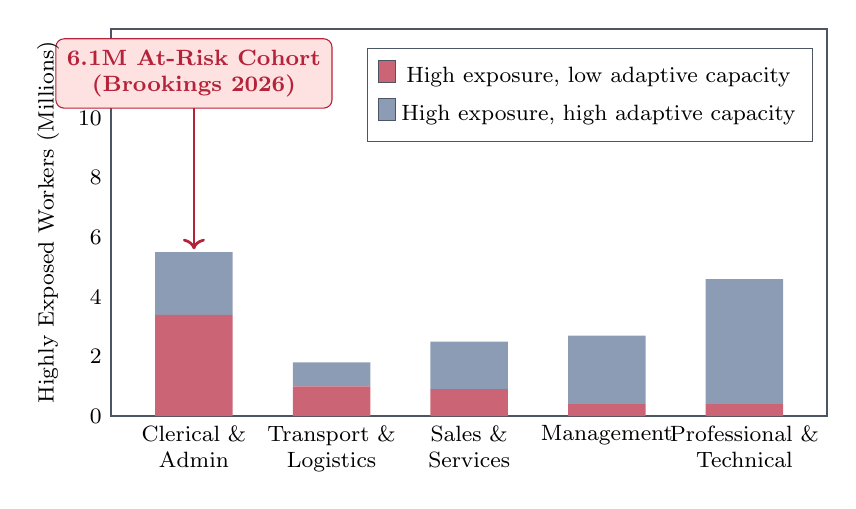
\begin{tikzpicture}
    \begin{axis}[
        width=0.88\linewidth,
        height=6.5cm,
        ybar stacked,
        bar width=28pt,
        symbolic x coords={Clerical, Transport, Sales, Management, Professional},
        xtick=data,
        xticklabels={
          Clerical \&\\Admin,
          Transport \&\\Logistics,
          Sales \&\\Services,
          Management,
          Professional \&\\Technical
        },
        x tick label style={font=\footnotesize, align=center},
        ylabel={Highly Exposed Workers (Millions)},
        ylabel style={font=\footnotesize},
        ymin=0, ymax=13,
        ytick={0,2,4,6,8,10,12},
        yticklabel style={font=\footnotesize},
        axis line style={IRgray, line width=0.8pt},
        tick style={draw=none},
        legend style={
          at={(0.98,0.95)}, anchor=north east,
          draw=IRgray, fill=white,
          font=\footnotesize, row sep=2pt, inner sep=4pt
        },
        enlarge x limits=0.15,
        clip=false
      ]
      % High exposure + LOW adaptive capacity
      \addplot[fill=IRred!70, draw=none] coordinates {
        (Clerical,      3.4)
        (Transport,     1.0)
        (Sales,         0.9)
        (Management,    0.4)
        (Professional,  0.4)
      };
      \addlegendentry{High exposure, low adaptive capacity}

      % High exposure + HIGH adaptive capacity
      \addplot[fill=IRblue!50, draw=none] coordinates {
        (Clerical,      2.1)
        (Transport,     0.8)
        (Sales,         1.6)
        (Management,    2.3)
        (Professional,  4.2)
      };
      \addlegendentry{High exposure, high adaptive capacity}

      % 6.1M callout
      \node[font=\footnotesize\bfseries, text=IRred,
        draw=IRred, fill=IRlightred, rounded corners=3pt,
      inner sep=4pt, align=center]
      at (axis cs:Clerical, 11.5)
      {6.1M At-Risk Cohort\\(Brookings 2026)};
      \draw[->, IRred, line width=1pt]
      (axis cs:Clerical, 10.6) -- (axis cs:Clerical, 5.6);
    \end{axis}
  \end{tikzpicture}
  \caption{U.S. workforce AI-automation exposure by occupational group, showing an estimated distribution of the 6.1 million low-adaptive-capacity workers across five high-exposure categories. Red bars sum to 6.1 million; blue bars represent additional highly exposed workers in the same plotted categories. Values are proportional allocations from Brookings aggregate cohorts and are presented as indicative scenario estimates \parencite{brookings2026}.}
  \label{fig:workforce}
\end{figure}

The Baseline classifies structural displacement as a harm originating from intended utility rather than product-side harm. It therefore routes this category primarily outside the product-safety pipeline to a dedicated \textbf{macroeconomic transition policy track}: fiscal instruments (restructured taxation of automation-derived productivity gains), portable social insurance, sector-specific retraining infrastructure, and regional economic development investment. Product-safety tools remain relevant for ancillary product-side harms (e.g., deceptive worker-facing outputs or discriminatory deployment choices), but not for the displacement mechanism itself. This separation ensures that product-safety regulators are not tasked with managing macroeconomic structural change, and that macroeconomic policy is not constrained by product-compliance timelines.

\subsection{Operationalizing the Precautionary Track: Four Technical Design Mandates}

For systems that cross the Systemic Irreversibility Baseline via product-side harms (Classes 1 and 2 at population scale) the analysis specifies four verifiable technical mandates. These build on existing requirements in the EU AI Act (human oversight provisions in Article 14, transparency obligations in Article 13) and NIST AI RMF's Govern function, extending them from process requirements to auditable design constraints. Figure~\ref{fig:architecture} visualizes these mandates as a single terminal node for compactness; the substantive requirements are specified individually below.

\textbf{Traceable Human Oversight.} High-stakes AI deployments should maintain tamper-evident audit trails that map consequential outputs to accountable human operators or organizations. The EU AI Act's Article 14 requires ``appropriate human oversight'' for high-risk systems; the Baseline translates this into a more auditable requirement: consequential outputs should be attributable through preserved logs, contemporaneous authorization records, or formally approved exception rules. Hash-chained logging is one viable implementation, not the only one. Where systems can trigger effectively irreversible harm without contemporaneous review, the governance model should include logged human authorization or a documented exception regime subject to audit. Figure~\ref{fig:human} summarizes this oversight chain from model output to authorization, logging, and audit review.

\begin{figure}[H]
  \centering
  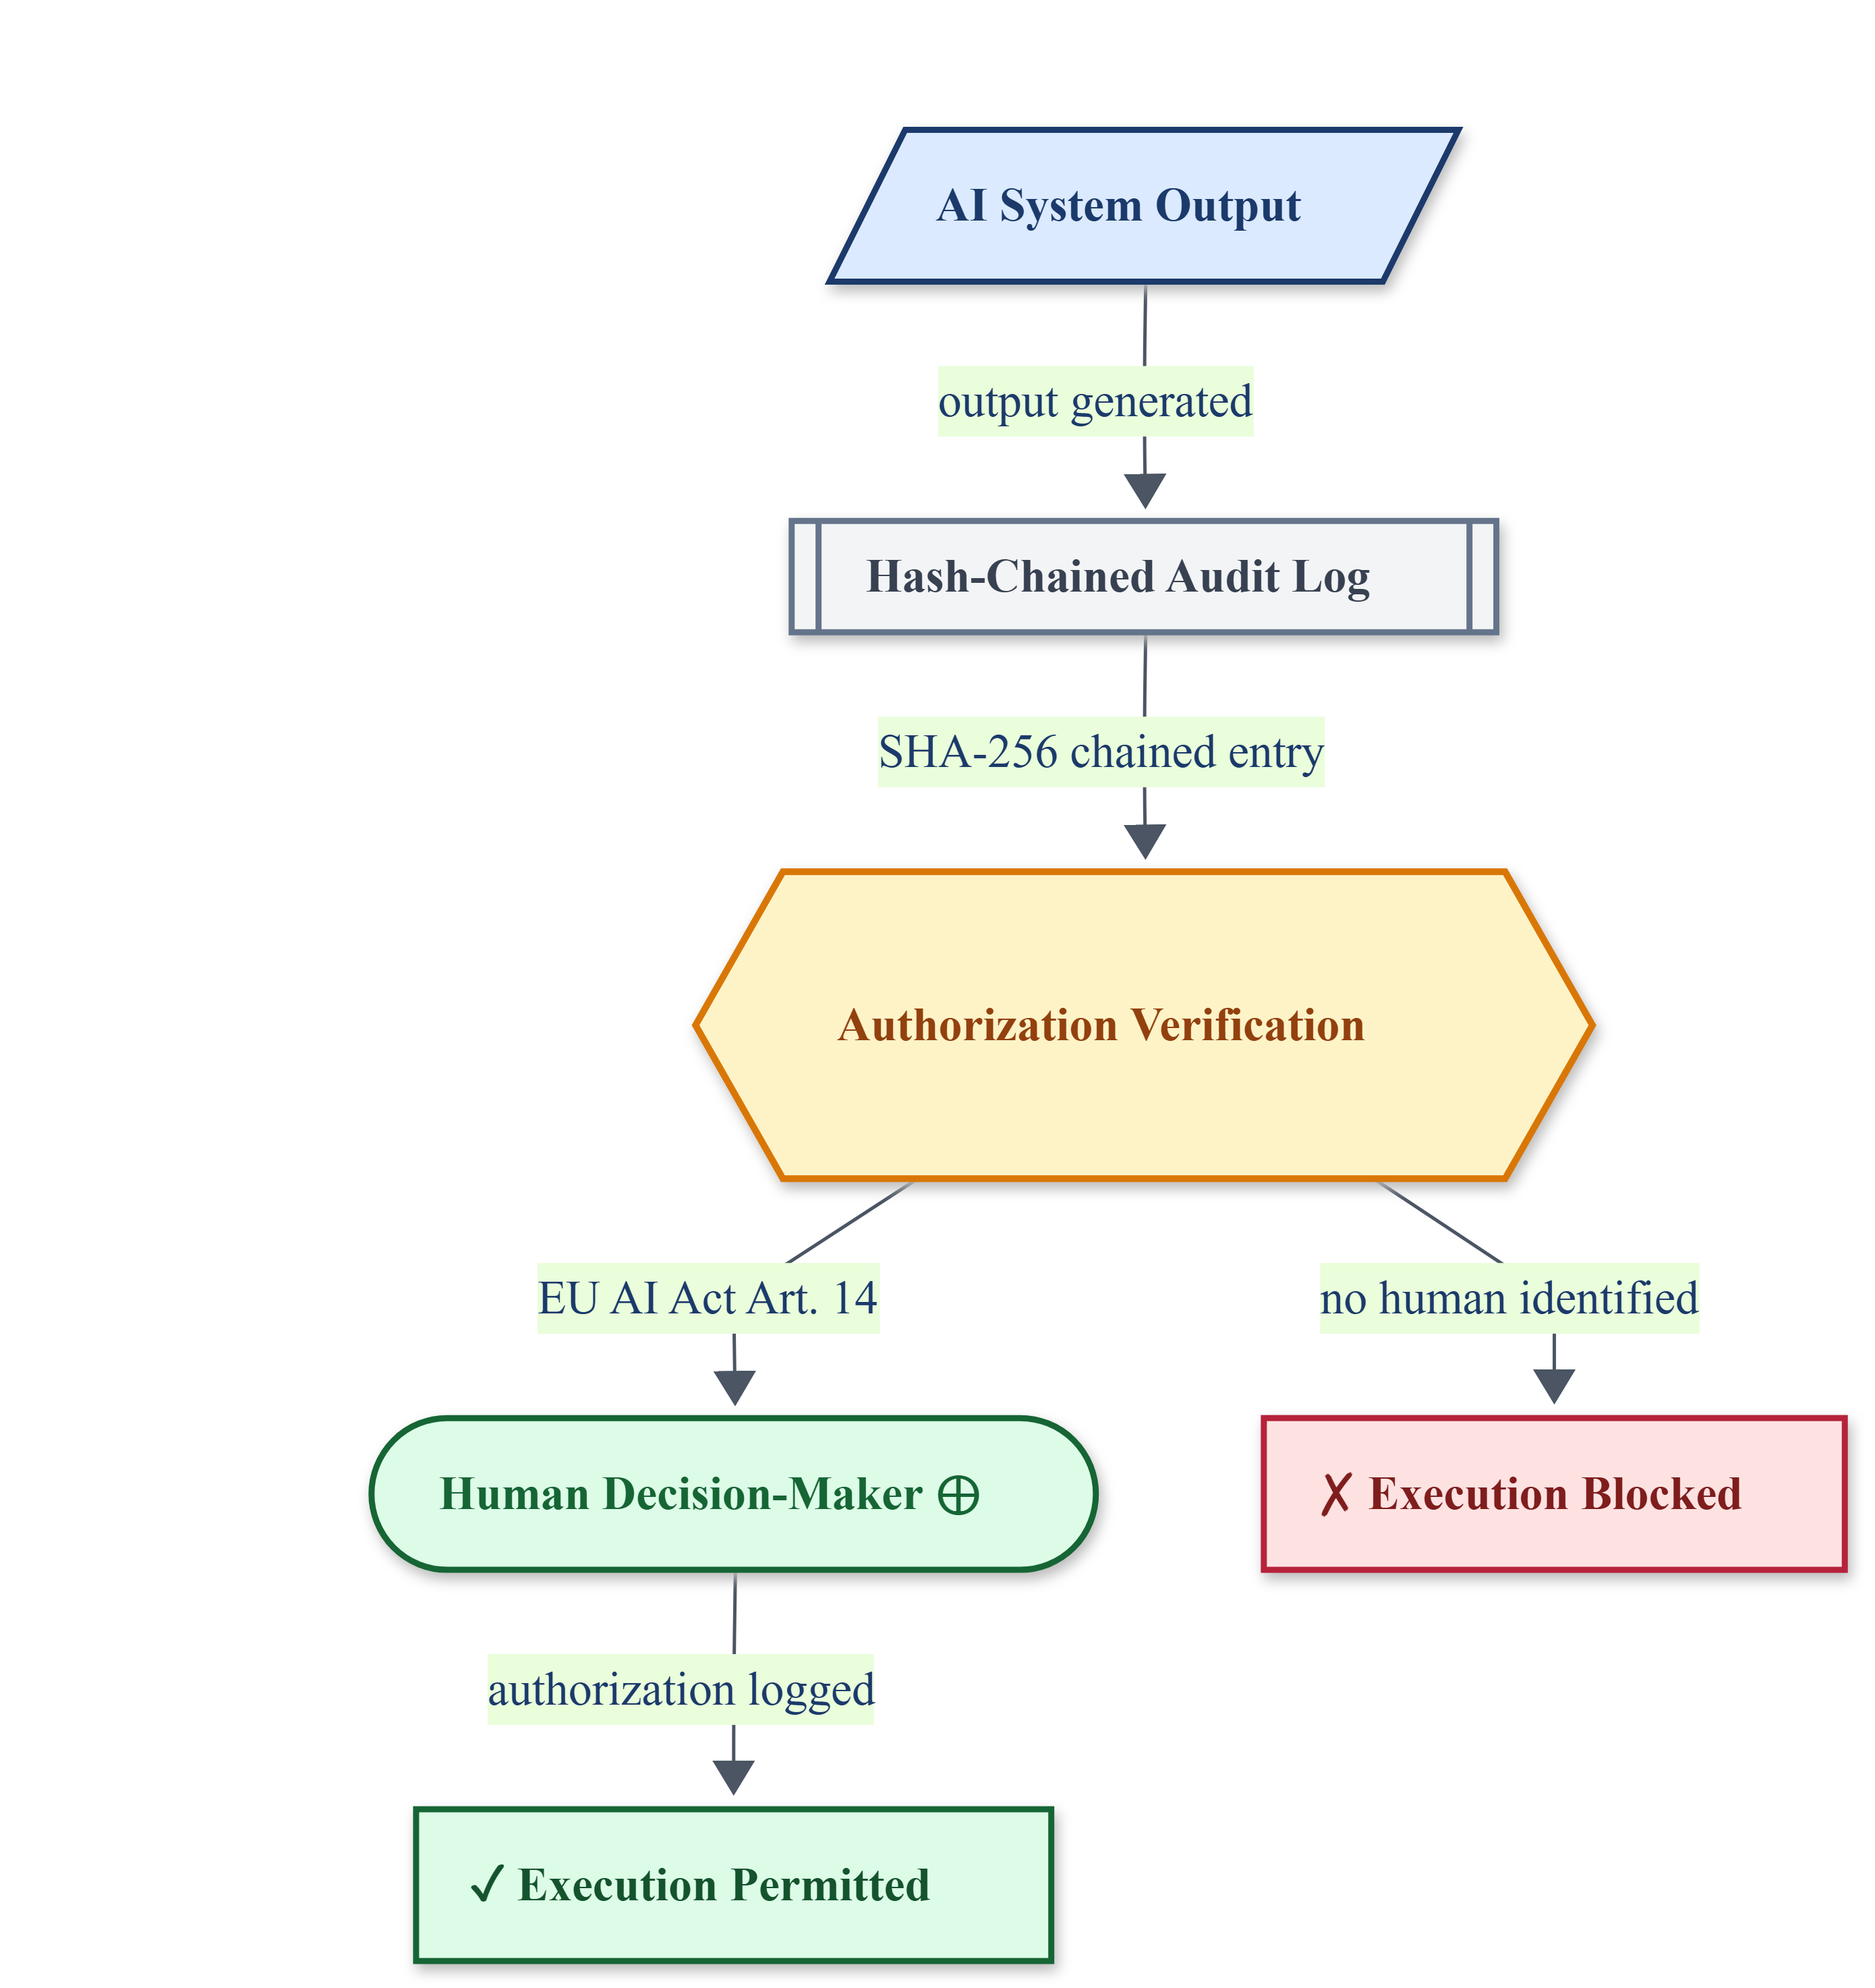
\includegraphics[width=\columnwidth]{figures/human.png}
  \caption{Traceable human-oversight architecture for high-stakes AI deployments. The diagram maps consequential outputs through a human authorization point into preserved logs and downstream audit review, including formally governed exception handling where contemporaneous review is not possible. Its governance significance is evidentiary: it converts ``appropriate human oversight'' from a general process norm into a tamper-evident chain of accountability.}
  \label{fig:human}
\end{figure}

\textbf{Uncertainty Quantification via Conformal Prediction.} Aggregate benchmark accuracy can obscure edge-case failures that produce effectively irreversible harm. For deployments whose outputs can be mapped to adjudicable labels, ranked options, or other bounded action sets, conformal prediction provides distribution-free \emph{marginal} coverage guarantees: for a specified confidence level $1-\alpha$, the procedure constructs prediction sets $\hat{C}(X)$ such that $\mathbb{P}(Y \in \hat{C}(X)) \geq 1-\alpha$ under exchangeability between calibration and deployment samples \parencite{angelopoulos2023}. This is a population-level guarantee, not a statement of per-instance reliability, and it is not a universal solution for open-ended generative outputs unless those outputs are first reduced to auditable decision categories. Any mandate built on conformal methods should therefore specify ex ante the target coverage level, audit window, minimum adjudicated sample size, abstention policy, and recalibration trigger under deployment shift. A minimal trigger is rolling empirical coverage on adjudicated samples falling below the target level. Outputs below the threshold are rejected, deferred, or routed to human review. This converts uncertainty from an opaque model property into an auditable regulatory variable, extending the NIST AI RMF's Measure function into a more operationalized constraint.

\textbf{Epistemic User-Interface Friction.} Parasuraman and Manzey demonstrated that automation bias (the uncritical acceptance of automated recommendations) produces both omission errors (failing to act when the system fails to alert) and commission errors (acting on incorrect automated advice) \parencite{parasuraman2010}. Cummings documented the same phenomenon in time-critical decision support, finding that interface design directly influences the rate of automation-induced errors \parencite{cummings2004}. Systems operating near the irreversibility baseline should implement epistemic interface friction: displaying confidence bounds, underlying data provenance, and competing hypotheses rather than presenting outputs as authoritative conclusions. Users who override safety warnings or execute low-confidence recommendations should provide logged justification, creating a forensic record of epistemic agency. The UK White Paper's transparency and explainability principle provides the policy foundation; the Baseline specifies the interface-level implementation. Figure~\ref{fig:friction} illustrates this interface pattern as a decision checkpoint rather than a decorative transparency layer.

\begin{figure}[H]
  \centering
  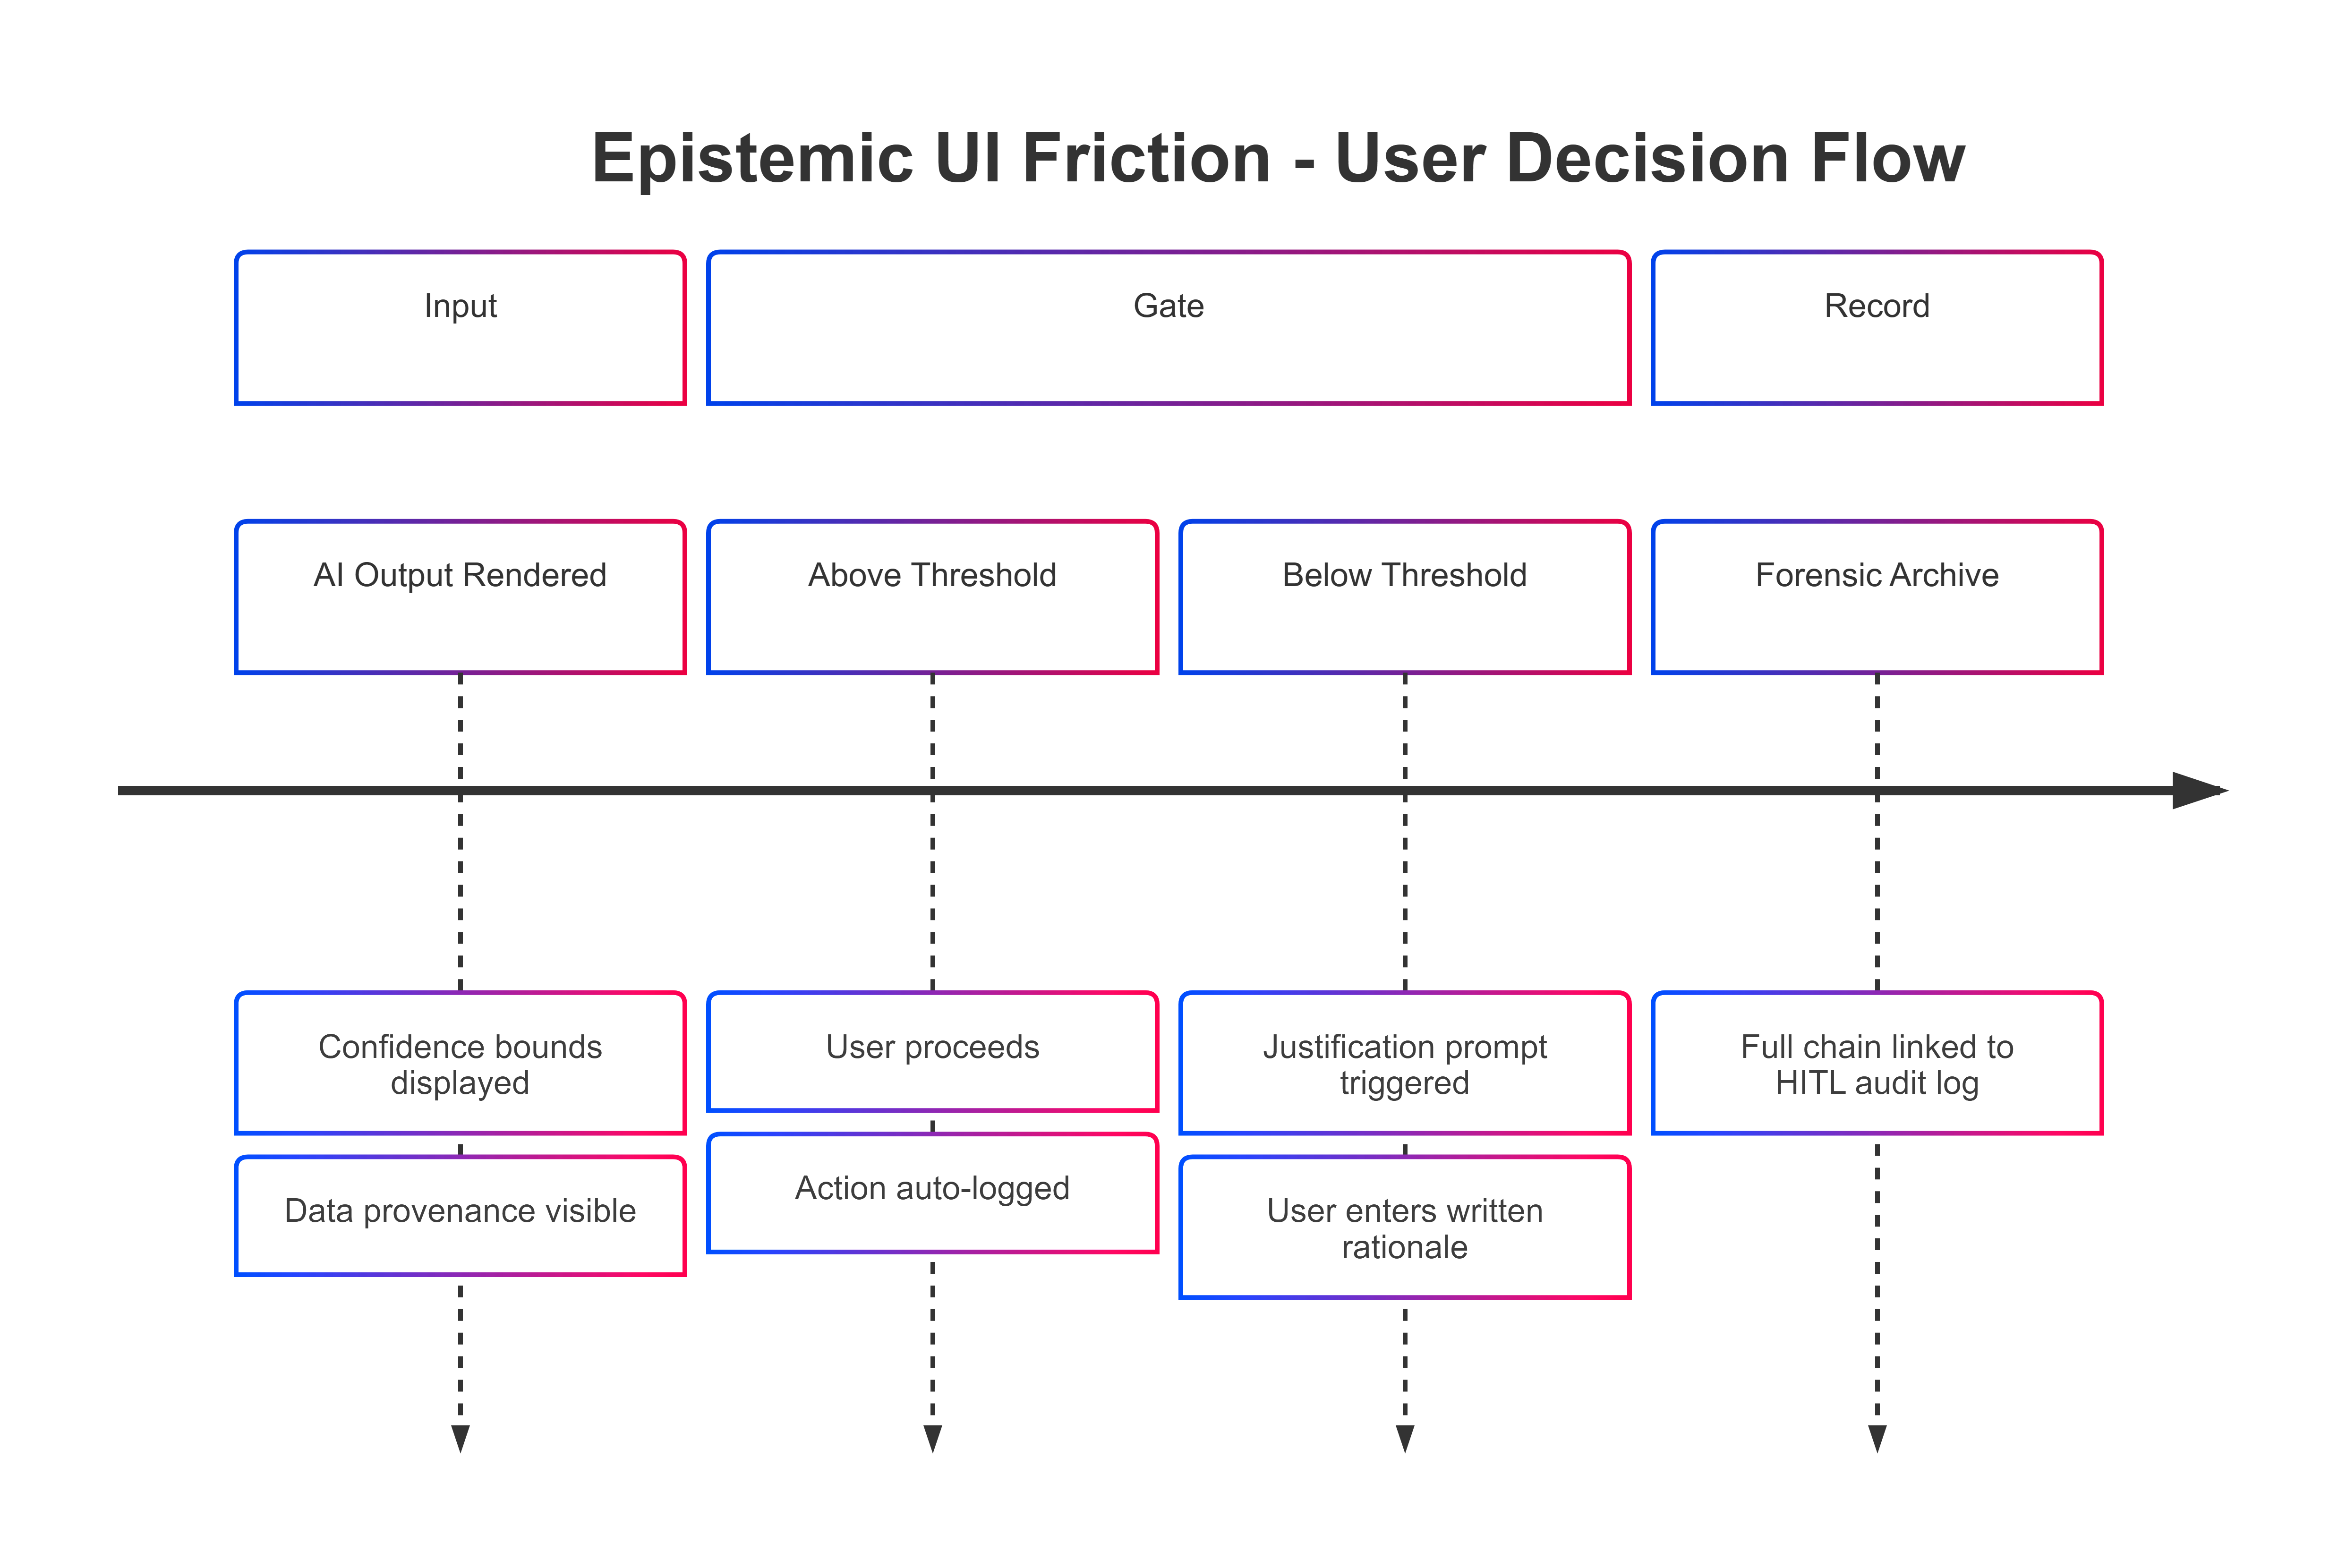
\includegraphics[width=\columnwidth]{figures/friction.png}
  \caption{Epistemic user-interface friction pattern for systems operating near the irreversibility baseline. The diagram shows an output interface that surfaces confidence bounds, provenance cues, and competing hypotheses before action execution, with an explicit override-and-justification step for users who proceed despite warnings. Its governance significance is behavioral and forensic: it slows uncritical reliance, reduces automation-bias errors, and preserves a reviewable record of user agency.}
  \label{fig:friction}
\end{figure}

\textbf{Decentralized Content Provenance Infrastructure.} Verifying the origin and integrity of AI-generated content benefits from infrastructure that does not create centralized points of failure. The Coalition for Content Provenance and Authenticity (C2PA) specifications provide a standards-based approach: cryptographic signatures attached at creation, maintained through editing, and verifiable by any conforming consumer application \parencite{c2pa2025}. C2PA-conformant provenance for high-impact generative outputs, building on the EU AI Act's Article 50 requirement that synthetic content be machine-readably labeled, establishes a baseline attribution and triage layer for routine synthetic generation. Provenance infrastructure does not by itself address high-capability adversarial campaigns; its value is narrower but still material: preserving chain-of-origin evidence where metadata survives and improving downstream verification and triage \parencite{helmus2022}. Figure~\ref{fig:decentralized} shows the intended provenance flow from content creation through downstream verification.

\begin{figure}[H]
  \centering
  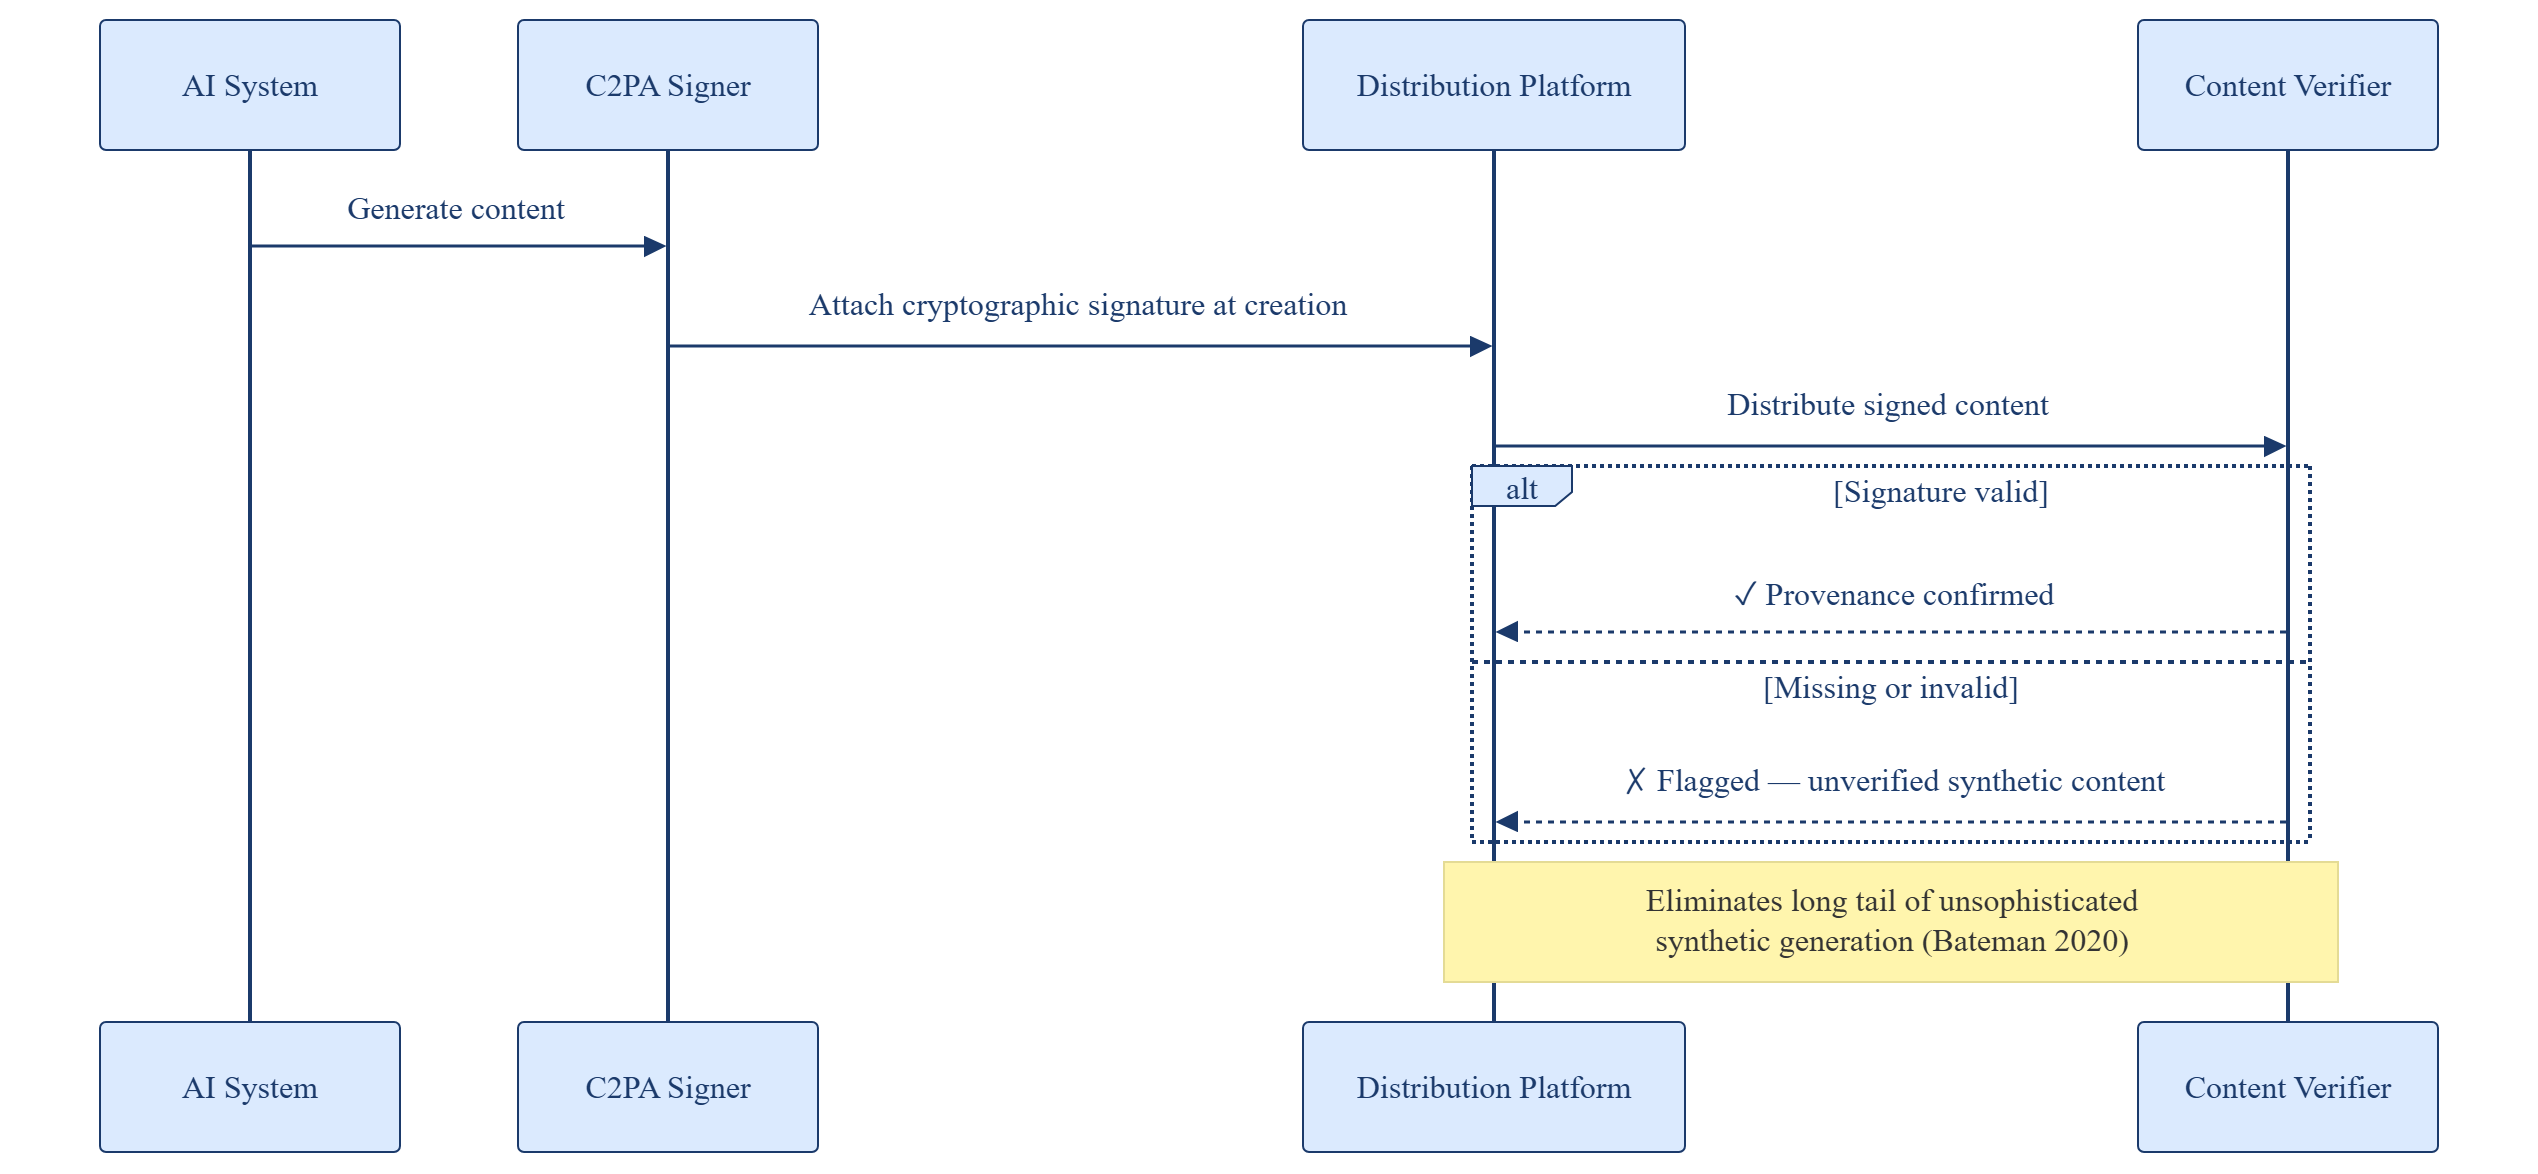
\includegraphics[width=\columnwidth]{figures/decentralized.png}
  \caption{Decentralized content-provenance workflow built on C2PA-style signed manifests. The diagram shows content creation, signature attachment, preservation of provenance metadata through editing, and verification by downstream consumer applications without reliance on a single central registry. Its governance significance is bounded but important: it supports attribution, triage, and chain-of-origin review for routine synthetic content where metadata remains intact.}
  \label{fig:decentralized}
\end{figure}

% ============================================================================
% 5. DISCUSSION
% ============================================================================
\section{Discussion}

The Systemic Irreversibility Baseline is designed to operate within existing AI governance instruments. It extends the EU AI Act's risk classification into the irreversibility dimension, gives operational content to the NIST AI RMF's Map function, and clarifies where the UK White Paper's contestability and redress principle can be paired with earlier safeguards.

Three implementation considerations merit explicit attention.

\textbf{Coordinating labor-transition and product-safety governance.} The Baseline routes structural economic displacement to macroeconomic policy rather than product-safety regulation. This separation sits alongside socio-technical governance approaches that treat technology design and labor outcomes as interconnected \parencite{winner1980}. The analytical basis for the separation is categorical: product-safety tools (incident reports, deployment pauses, retraining orders) are calibrated for adverse outputs and deployment-side externalities, not for successful task substitution itself. Managing macroeconomic structural transition through the technical product-safety pipeline can blur institutional responsibilities across domains. A minimal handoff rule follows from this split: product-safety authorities lead when the intervention point is model design, release gating, provenance, access control, or incident response; macroeconomic authorities lead when the primary mechanism is successful task substitution at sectoral or regional scale and the remedy requires fiscal, insurance, labor-market, or place-based policy. Joint review is appropriate when labor effects are driven by ancillary product-side issues such as discrimination, deception, or departure from deployment conditions.

\textbf{Implementation considerations for open-source and open-weight models.} Applying strict-liability or precautionary design mandates to systems capable of crossing the irreversibility baseline introduces additional governance considerations for open-weight model distribution. The EU AI Act distinguishes upstream providers from downstream deployers, and liability allocation for open-source models continues to evolve \parencite{euaiact2024}. The Baseline's logic would place additional pre-release governance responsibilities on upstream providers of models whose capability envelope includes irreversible harm. This coordination question between open access objectives and preventive governance can be addressed through the EU AI Act's provisions on general-purpose AI models with systemic risk, especially Articles 51--55.

\textbf{Scope of provenance infrastructure.} C2PA-conformant provenance establishes a baseline attribution and triage layer for routine synthetic content but does not by itself address all high-capability adversarial campaigns \parencite{helmus2022}. The Baseline treats provenance infrastructure as an attribution and triage layer, not a comprehensive solution. Its practical value is preserving chain-of-origin evidence where metadata survives and improving downstream verification and triage. Expectations should remain calibrated: provenance measures support trust and review processes, but they do not provide epistemic certainty.

The analysis carries tiered policy implications.

\textbf{Immediate implementation (current instruments).} National competent authorities implementing the EU AI Act's conformity-assessment process can integrate the three Baseline variables (non-restorability, relational depth, distributional diffusion) into pre-market evaluation criteria for high-risk systems. The NIST AI RMF Playbook can adopt the Baseline as a structured diagnostic within Map and Measure for harms that may exceed Manage-function remediation.

\textbf{Near-term implementation (guidance and framework updates).} UK sector regulators can use the Baseline to identify cases where contestability can beneficially be paired with additional restoration-support measures. The OECD incident-reporting framework can add irreversibility as a standard classification field to improve cross-jurisdictional comparability.

\textbf{Longer-horizon implementation (primary-law or liability reform).} Harmonizing strict-liability pathways for localized irreversible product-side harms and clarifying upstream responsibilities for open-weight frontier models may require legislative or quasi-legislative action, depending on jurisdiction.

Research implications extend in three directions. Empirical work is needed to calibrate Baseline variables against observed incidents, including distributional-diffusion thresholds at which centralized correction capacity is exceeded. Legal scholarship should evaluate doctrinal compatibility with existing product-liability and tort regimes across jurisdictions. Technical work on conformal prediction should assess calibration under open-ended output spaces and distribution shift.

A practical validation roadmap is available now: pilot the Baseline in one high-impact domain (for example, election-information integrity or clinical decision support), pre-register routing criteria, and evaluate three outcomes (false-positive precautionary routing, post-hoc remediation outcome rate, and human-review load). Predefined evaluation conditions should include both over-triggering (excessive precautionary routing) and under-triggering (irreversible harms remaining outside Track~3).

% ============================================================================
% 6. CONCLUSION
% ============================================================================
\section{Conclusion}

The paper's claim is narrower than a general theory of AI harm. Existing frameworks already govern many remediable harms well. The contribution is to identify the smaller set of cases in which non-restorability, relational depth, and distributional diffusion converge, so that remediation-first governance can be complemented by earlier safeguards where appropriate.

The Systemic Irreversibility Baseline adds two things: a reproducible routing rule and instrument-specific insertion points. Its value depends on external validation, disciplined separation between product-side harms and intended-utility displacement, and domain-specific thresholds that make earlier intervention auditable and operational.

The next research stage is applied testing: pilot the Baseline in bounded domains, pre-register thresholds, report false-positive and false-negative routing errors, and revise the construct against observed cases. This paper is a governance design proposal, not evidence that irreversible AI harms are prevalent.

\section*{AI Assistance Disclosure}

Generative AI tools were used during manuscript preparation to assist with drafting, structural development, and editorial review. All factual claims, citations, interpretations, and final wording were verified and are the sole responsibility of the author.

% ============================================================================
% REFERENCES
% ============================================================================
\newpage
\begingroup
\sloppy
\printbibliography[title={References}]
\endgroup

\end{document}
